\documentclass[notitlepage, a4paper, 11pt]{article}

\usepackage{geometry}
\geometry{
	a4paper,
	total={170mm,257mm},
	left=20mm,
	top=20mm,
}
\usepackage{ gensymb }
\usepackage{wrapfig}
\usepackage{xcolor}
\usepackage{graphicx}
\usepackage{amsmath}
\usepackage{listings}
\usepackage{xcolor}
\usepackage{minted}
\usepackage{tikz}
\usepackage[european resistors]{circuitikz}
\usepackage{caption}
\usepackage{subcaption}
\usepackage{hyperref}
\hypersetup{
	pdfborder = false,
	colorlinks=true,
	linkcolor=black,
	filecolor=black,      
	urlcolor=blue,
	pdftitle={Overleaf Example},
	pdfpagemode=FullScreen,
}
\title{Frequency Response Measurements\\
	\large Laboratory IV}
\author{Patrycja Nazim, Adrian Król, Gabriel Ćwiek, Kamil Chaj}
\date{}

\begin{document}
	\maketitle
	\section{Goal of the exercise}
	
	The objective of the exercise is to acquaint oneself with the techniques for determining the frequency responses of selected circuits, specifically filters. This objective is accomplished by measuring the response of the circuits when subjected to sinusoidal inputs of varying frequencies. Through this process, participants can gain familiarity with the behavior and characteristics of the circuits under different frequency conditions, allowing for a better understanding of their frequency response properties.
	
	\section{Frequency response}
	
	The frequency response of a system or circuit describes its behavior in response to different frequencies of input signals. It shows how the system amplifies or attenuates specific frequencies within a given range. In the context of filters, the frequency response indicates which frequencies are passed or attenuated by the filter. Analyzing the frequency response helps assess a filter's performance, determine its suitability for specific applications, and make informed decisions about its usage in electronic systems.
	
	\begin{equation}
		H(s) = \dfrac{V_{out}(s)}{V_{in}(s)}
	\end{equation}
	
	\section{Course of measurements}
	
	In this lab, we explored the frequency response characteristics of different filters by measuring and analyzing their voltage outputs. The lab focused on three specific circuits: an RC integrating circuit (low-pass filter), a third-order low-pass filter, and a resonant circuit RLC.
		
	We began by setting the frequency range from 1 kHz to 10 kHz with a step size of 1 kHz for the RC integrating circuit. We measured the voltage output at each frequency point and recorded the results. Then, we adjusted the frequency range to 10 kHz to 20 kHz with a step size of 2 kHz and repeated the voltage measurements.
	
	\begin{figure}[H]
		\centering
		\begin{circuitikz}[scale = 0.7, transform shape]
			\draw (0,0) node[bnc](B1) {CON11}
			to[R, l=$R_{11}$, a=1.5k$\Omega$] (3,0)
			to[C, l=$C_{11}$, a=47nF] (3,-2)
			node[ground] {}
			;
			\draw (3,0) 
			to[short] (4.5,0)
			node[bnc, xscale=-1](B2){\scalebox{-1}[1]{CON12}}
			;
			\draw node[ground] at (B1.shield) {};
			\draw node[ground] at (B2.shield) {};
		\end{circuitikz}
		\caption{RC low-pass filter}
	\end{figure}
	
	Next, we moved on to the third-order low-pass filter. We set the frequency range from 1 kHz to 10 kHz with a step size of 1 kHz and measured the voltage output at each frequency point. We recorded the results and adjusted the frequency range to 10 kHz to 20 kHz with a step size of 2 kHz. We repeated the voltage measurements for this extended frequency range.
	
	\begin{figure}[H]
		\centering
		\begin{circuitikz}
			\ctikzset{bipoles/length = 10mm}
			\ctikzset{font = \tiny}
			\node [bnc] at (0, 0)(CON1) {CON31};
			\node [bnc, xscale=-1] at (8, 0)(CON2) {\ctikzflipx{CON32}};
			\draw (CON1.hot) -- (1.5, 0)
			to[C, l2=$C_{31}$ and 1$\mu$F, l2 halign=c, l2 valign=a] (1.5, -2) node[tlground]{};
			\draw (1.5, 0) -- (3, 0)
			to[C, l2=$C_{32}$ and 330nF, l2 halign=c, l2 valign=c] (3, -2) node[tlground]{};
			\draw (3, 0)
			to[L, l2=$L_{31}$ and 680$\mu$H, l2 halign=c, l2 valign=c] (4.5, 0)
			to[C, l2=$C_{34}$ and 330nF, l2 halign=c, l2 valign=c] (4.5, -2) node[tlground]{};
			\draw (4.5, 0) -- (6, 0)
			to[C, l2=$C_{34}$ and 330nF, l2 halign=c, l2 valign=c] (6, -2) node[tlground]{};
			\draw (6, 0) -- (CON2.hot);
			\draw (7.5, 0) 
			to[nopbc] (7.5, -1)
			to[R, l2^=$R_{31}$ and 51$\Omega$, l2 halign=c, l2 valign=c, bipoles/length = 8mm] (7.5, -2) node[tlground]{};
		\end{circuitikz}
		\caption{III-order low-pass filter}
	\end{figure}
	
	Finally, we worked with the resonant circuit RLC. We set the frequency range from 1 kHz to 8 kHz with a step size of 1 kHz and measured the voltage output at each frequency point. We recorded the results and adjusted the frequency range to 8 kHz to 10 kHz with a step size of 0.2 kHz. We then adjusted it further to 10 kHz to 20 kHz with a step size of 2 kHz and repeated the voltage measurements for each frequency range.
	
	\begin{figure}[H]
		\centering
		\begin{circuitikz}[scale = 0.7, transform shape]
			\node [bnc] at (0,0) (CON41) {CON41};
			\draw (CON41.hot) to[short, -*]
			(1,0) -- (3,0) to[nopb, l_=JP43] (4,0);
			\draw (1,0) -- (1,-2) to[R, l2=$R_{42}$ and $1.1k\Omega$, l2 halign=c, l2 valign=b] (3,-2)
			to[nopb, l_=JP42] (4,-2) -- (4, 0);
			\draw (1,-2) -- (1,-4) to[R, l2=$R_{41}$ and $3.3k\Omega$, l2 halign=c, l2 valign=b] (3,-4)
			to[nopb, l_=JP41] (4,-4) -- (4, -2);
			\draw (4,0) to[short, -*] (5,0)
			to[C, l2=$C_{41}$ and 33nF, l2 halign=c, l2 valign=c] (5,-2) 
			to[L, l2=$L_{41}$ and 10mH, l2 halign=c, l2 valign=c] (5,-4) node[ground] {};
			\draw (5, 0) to (6, 0) node[bnc, xscale=-1, anchor=zero](CON42){\ctikzflipx{CON42}};
		\end{circuitikz}
		\caption{Resonant RLC circuit}
	\end{figure}
	
	By conducting these measurements and analyzing the results, we gained a deeper understanding of the frequency response behaviors of different filters and their responses to varying frequencies.
		
	\section{Data processing}
	\begin{wrapfigure}{r}{0.4\textwidth}
		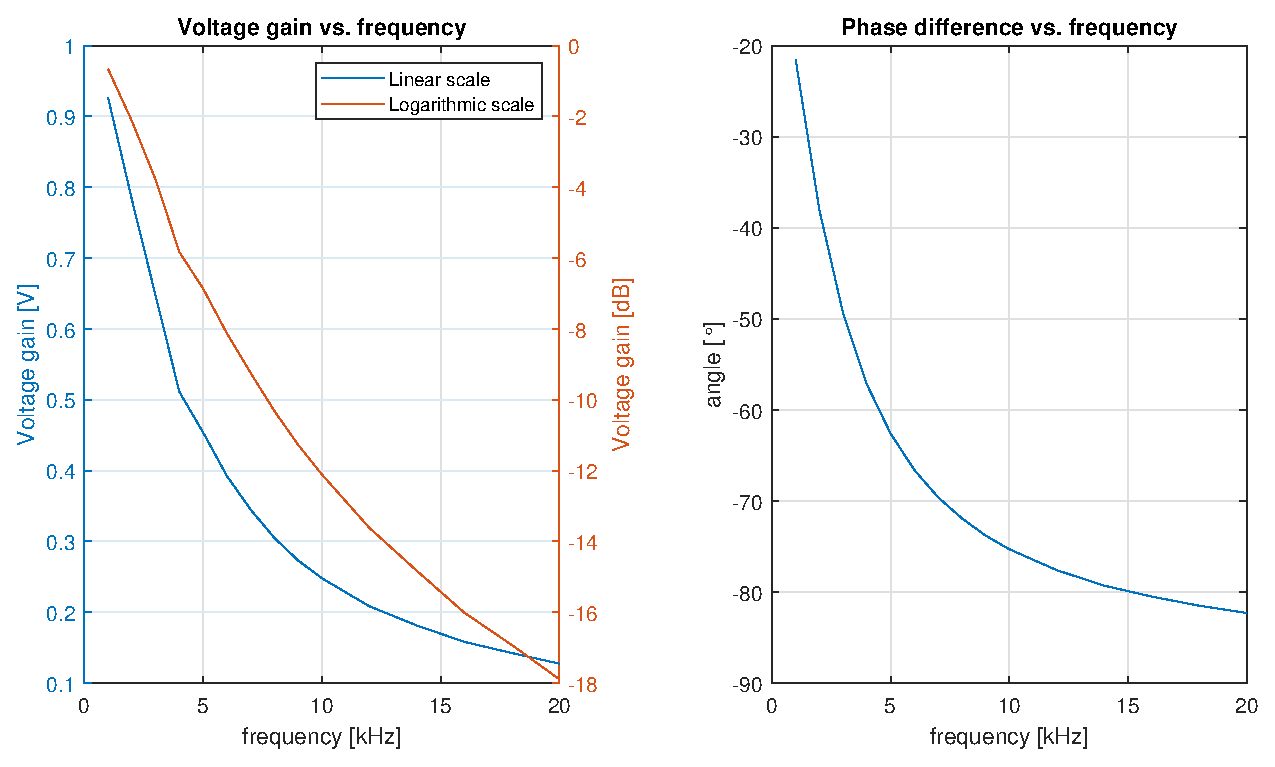
\includegraphics[width=0.4\textwidth]{../Matlab/img/11.eps}
		\caption{Example}
		\label{fig:example}
	\end{wrapfigure}
	
	Source code for this section can be found in Appendix \ref{sec:appendix}
	
	First step in finding amplitude-frequency characteristics was calculating gain in Volts
	
	\begin{equation}
		\text{Voltage gain [V]} = \dfrac{V_{\text{CON2}}}{V_{\text{CON1}}}
	\end{equation}
	
	then we calculated voltage gain in decibels
	
	\begin{equation}
		\text{Voltage gain [dB]} = 20 \log_{10}(V_{\text{gain}})
	\end{equation}
	
	Voltage gain is on the left plot in figure \ref{fig:example}, vertical blue axis represents scale in volts and orange axis decibel scale.
	
	Phase-frequency characteristics didn't require any calculation and is simply plotted on the right plot in figure \ref{fig:example}.
	
	\section{Characteristics analysis}
	
	The Low Pass Filter passes low frequencies and blocks high frequencies.	It only allows low frequency signals from 0Hz to its cut-off frequency ($f_c$) point to pass while blocking those any higher. $f_c=\dfrac{1}{2\pi RL RC}$ Looking at the voltage gain vs frequency graph we are able to spot point where the characteristic " breaksdown" and starts going rapidly down.
	
	\begin{figure}[H]
	\centering
	\begin{subfigure}{0.49\textwidth}
		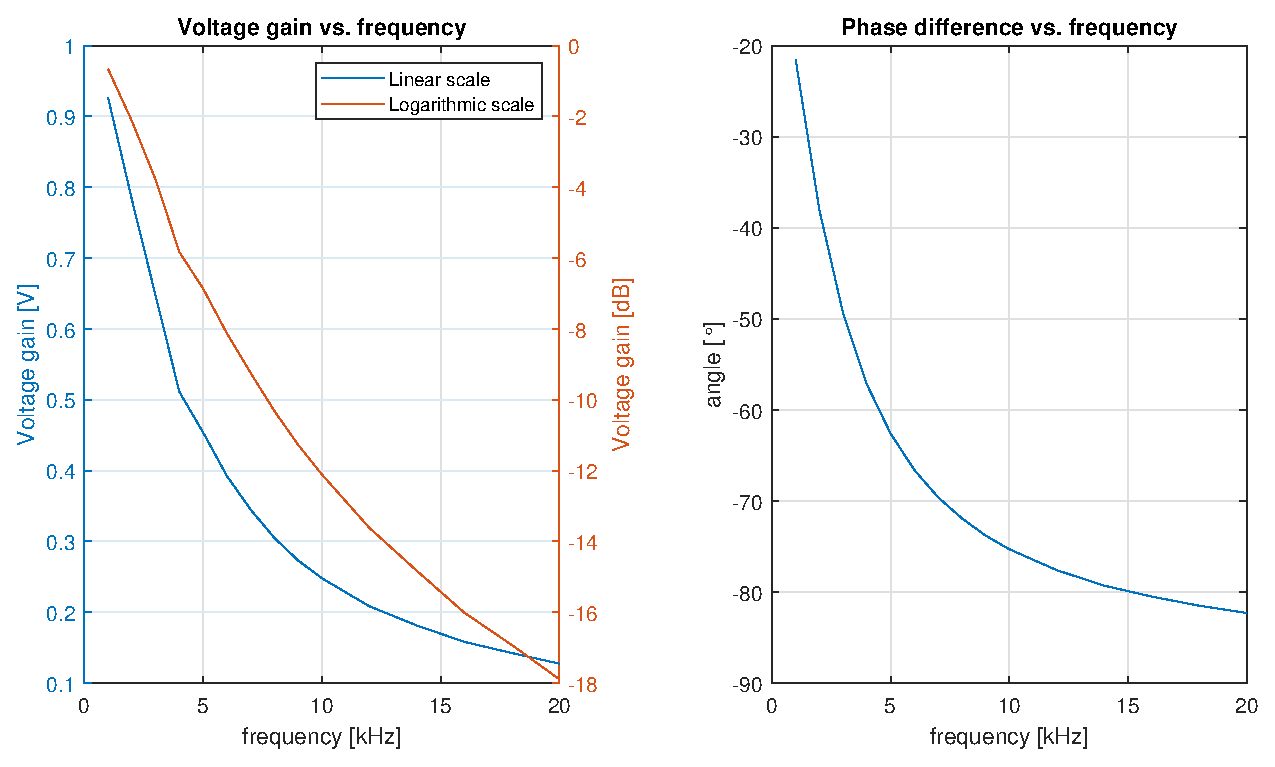
\includegraphics[width=\textwidth]{../Matlab/img/11.eps}
		\caption{RC low-pass filter}
	\end{subfigure}
	\hfill
	\begin{subfigure}{0.49\textwidth}
		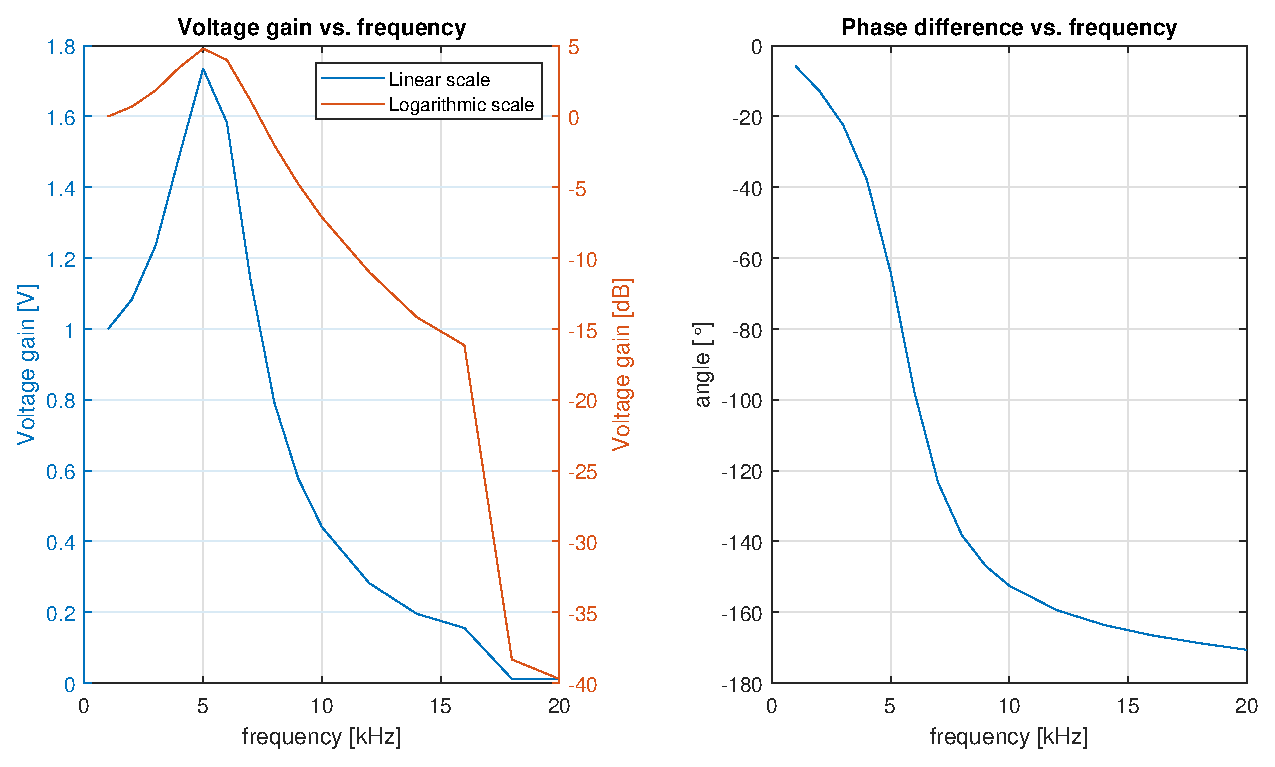
\includegraphics[width=\textwidth]{../Matlab/img/12.eps}
		\caption{III-order low-pass filter}
	\end{subfigure}
	\caption{Frequency response of low-pass filters circuit}
	\end{figure}
	
	The response of course starts at zero, reaches a maximum value in the vicinity of the natural resonant frequency, and then drops again to zero as $\omega$ becomes infinite. On our gain vs frequency graph we are able to notice the start of the characteristic taking place, before reaching a maximum value in the vicinity of the natural resonant frequency.
	
	\begin{figure}[H]
		\centering
		\begin{subfigure}{0.49\textwidth}
			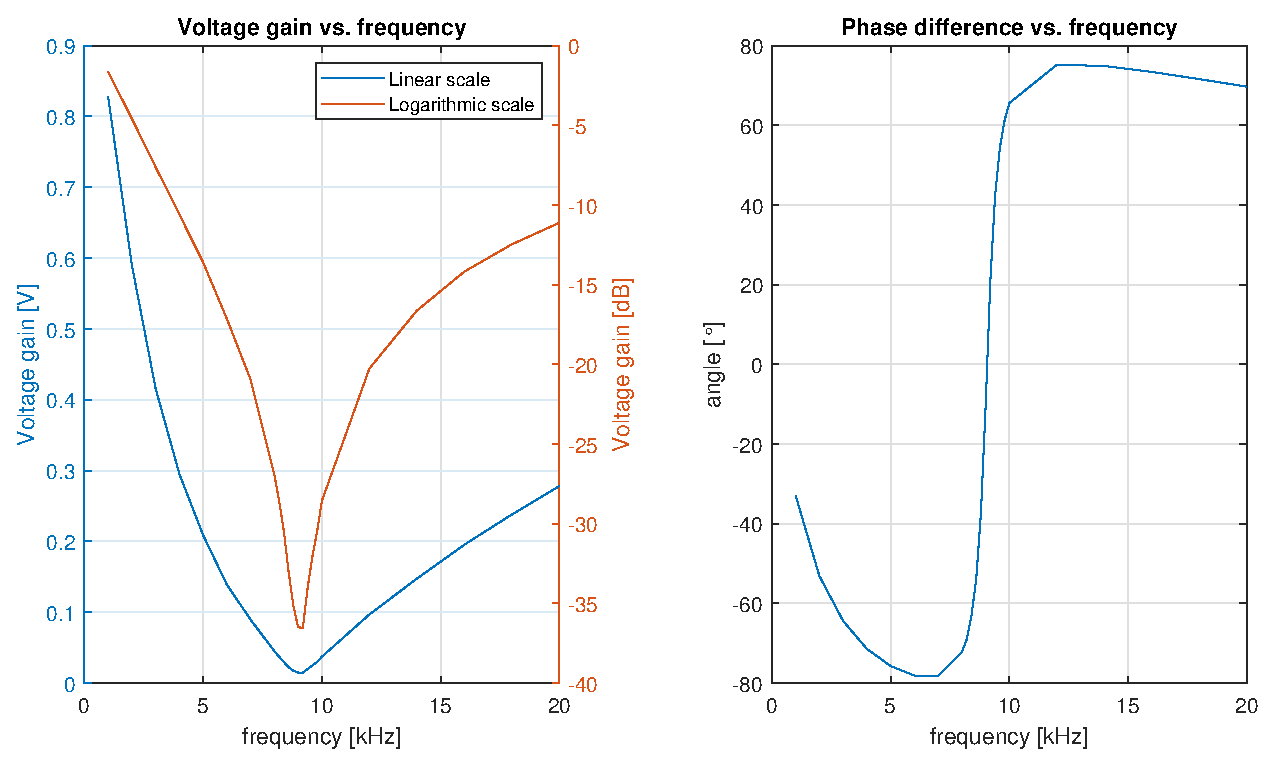
\includegraphics[width=\textwidth]{../Matlab/img/131.eps}
			\caption{with JP41}
		\end{subfigure}
		\hfill
		\begin{subfigure}{0.49\textwidth}
			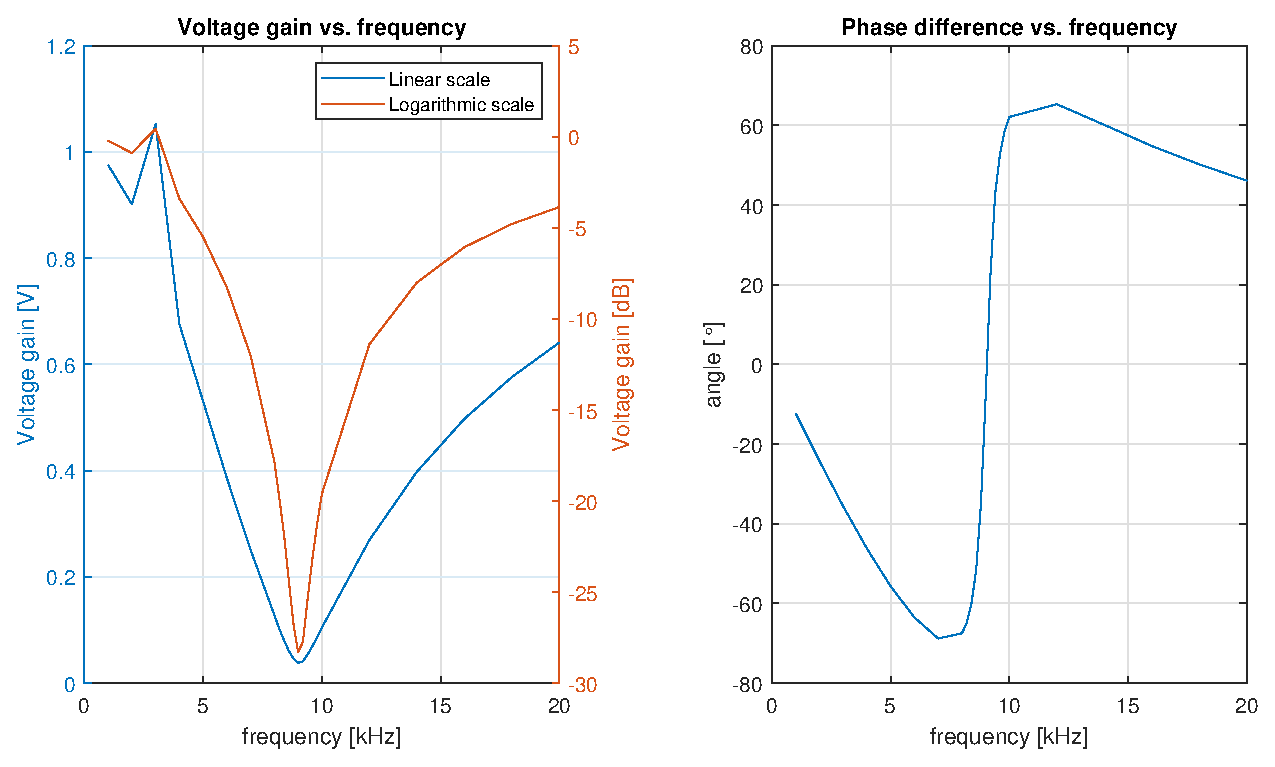
\includegraphics[width=\textwidth]{../Matlab/img/132.eps}
			\caption{with JP42}
		\end{subfigure}
		\caption{Frequency response of Resonant RLC circuit}
	\end{figure}
	\section{Conclusions}
	
	Measuring frequency responses lets us analyze chosen circuits(filters) in its frequency domain.	It also describes the steady-state response of a system to sinusoidal inputs of varying frequencies. From the measurements of the amplitude(ratio of voltages) and phase(in radians or degrees) of the output as a function of input frequency	we are able to do simpler analysis of more complex systems like the filters in our laboratories. The frequency response is closely related to the transfer function in linear systems, which is the Laplace transform of the impulse response. Using plots graphs to draw characteristics of the quantities we have measured gives us a great way to look at frequency response. Once a frequency response has been measured (e.g., as an impulse response), provided the system is linear and time-invariant, its characteristic can be approximated with arbitrary accuracy by a digital filter. Similarly, if a system is demonstrated to have a poor frequency response, a digital or analog filter can be applied to the signals prior to their reproduction to compensate for these deficiencies.	
	
	\newpage
	\appendix
	\section{Appendix}\label{sec:appendix}
	\href{https://github.com/kamilix2003/CT_labs}{GITHUB repository}
	\inputminted{matlab}{../Matlab/main.m}
	\inputminted{matlab}{../Matlab/import_csv.m}
	\inputminted{matlab}{../Matlab/characteristics.m}
\end{document}